% Input common header
\documentclass[xcolor=dvipsnames]{beamer}

\usecolortheme[named=Blue]{structure}
\setbeamertemplate{itemize items}[circle]

\usepackage{smartdiagram}


\author{Dr. Paul Larsen}
\date{\today}



\title{Discrete Geometry for Risk and AI}
\begin{document}
\maketitle


\begin{frame}
\frametitle{Why discrete geometry?}

\begin{itemize}
\item Recent history: Dissatisfaction with deep learning, only ``curve fitting'', alternatives via \emph{causal graphical models} \cite{pearl2019limitations}
\item Less recent history: graphical models among first non-rules based AI approaches \cite{darwiche2009modeling}
\item Geometrical formulations of statistical objects, e.g. graphical models and probability polytopes\newline
\end{itemize}

\end{frame}


\begin{frame}
  \frametitle{Directed graphical model: university admission gender bias}
  \framesubtitle{Simpson paradox preview}

  \begin{figure}[ht]
    \centering
            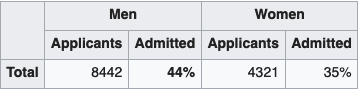
\includegraphics[height=0.15\textwidth]{graphics/berkeley} 
            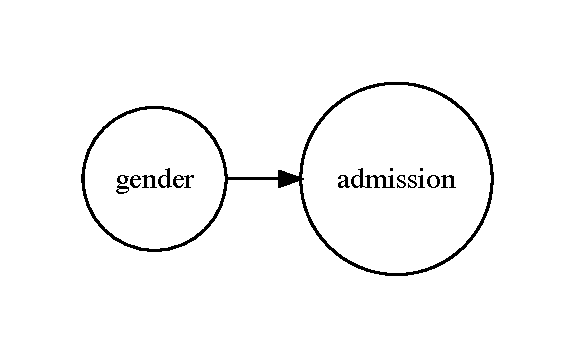
\includegraphics[height=0.4\textwidth]{graphics/admission_original}
       
    \end{figure}
    Sources: \cite{simpson-wikipedia} \cite{freedman1998statistics}
\end{frame}

\begin{frame}
  \frametitle{Directed graphical model: university admission gender bias}
  \framesubtitle{Simpson paradox preview}

  \begin{figure}[ht]
    \centering
            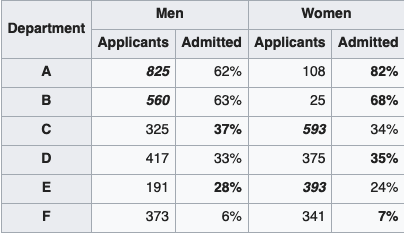
\includegraphics[height=0.35\textheight]{graphics/berkeley_later} 
            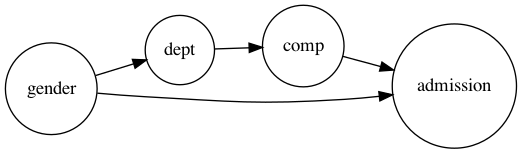
\includegraphics[height=0.35\textheight]{graphics/admission_later}
    \end{figure}
    Sources: \cite{simpson-wikipedia} \cite{Bickel398}
\end{frame}


\begin{frame}
\frametitle{Directed graphical model: hit rate for insurance quotes}
\begin{itemize}
  \item product type: financial, liability, property
  \item days: number of days to generate quote
  \item rating: measure of premium paid expected claims
  \item hit: 0 if quote refused, 1 if accepted
\end{itemize}
\begin{figure}[ht]
  \centering
  \includegraphics[height=0.7\textheight]{graphics/hit}
\end{figure}
\end{frame}


\begin{frame}
\frametitle{Undirected graphical model: credit default risk \cite{filiz2012graphical}}

\begin{itemize}
  \item Nodes take values 0 (healthy) or 1 (default)
  \item Industry nodes connect to other industry nodes
  \item Individual firm nodes connect only to corresponding industry node
\end{itemize}
\begin{figure}[ht]
  \centering
  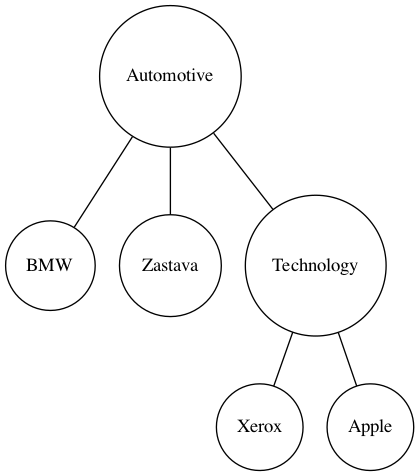
\includegraphics[height=0.6\textheight]{graphics/credit_default}
\end{figure}
\end{frame}


\begin{frame}
\frametitle{Graph definitions}
\begin{definition}
A \emph{graph} is a pair of sets $(V, E)$, where $V$ is called the set of \emph{vertices} (or \emph{nodes}) and $E$ is called the set of \emph{edges}, such that the set of edges corresponds injectively to pairs of vertices. \newline
\end{definition}

\emph{Notes}
\begin{itemize}
\item Typically `pairs of vertices` does not include self-pairs, but this can be relaxed, leading to graphics with with loops.
\item The injectivity requirement can also be relaxed, leading to \emph{multigraphs}.
\end{itemize}
\end{frame}


\begin{frame}
\frametitle{Graphical models}
\begin{definition}
(Informal) A graphical model is a graph whose nodes represent variables and whose edges represent direct statistical dependencies between the variables.\newline
\end{definition}

\emph{Why graphical models?}
\begin{itemize}
\item For probability distributions admitting a graphical model representation, then graph properties (\emph{d-separation}) imply conditional independence relations.
\item Conditional independence relations reduce the number of parameters required to specify a probability distribution.
\item Graphical models come in two flavors depending on their edges: directed (aka \emph{Bayesian Networks}) and undirected (aka \emph{random Markov fields}.
\end{itemize}
\end{frame}


\begin{frame}
\frametitle{Directed acyclic graphs}

\begin{definition}
A graph $G = (V, E)$ is a \emph{directed acyclic graph} (denoted also \emph{DAG}) if all edges have an associated direction, and no edge path consistent with the directions forms a cycle.\newline

If there is a directed path from $X_i$ to $X_j$, then $X_i$ is called a \emph{parent} of $X_j$, and $Pa(X_j) \subseteq V$ is the set of all parents of $X_j$.
\end{definition}

\begin{definition}
  If $X = (X_1, \ldots, X_m)$ admits a DAG $G$, then $X_G$ is a \emph{DAG model} if the distribution of $X$ decomposes according to $G$, i.e.

  \begin{equation*}
    P(X) = \prod_{i \in \{1, \ldots, m\}} P(X_i | Pa(X_i))
  \end{equation*}
\end{definition}
\end{frame}


\begin{frame}
  \frametitle{Example: Karma and weight-lifting}
  Take $K$ to be your Karma, $H$ to be the hours you spend in the gym lifting weight each day, and then $W$ be the weight you can bench press on a given day. For simplicity, all random variables are binary.\newline
  
  \begin{tabular}{rrr}
\toprule
 karma &  hours &  weight \\
\midrule
     1 &      0 &       1 \\
     1 &      1 &       1 \\
     0 &      1 &       0 \\
     1 &      0 &       1 \\
     1 &      0 &       1 \\
\bottomrule
\end{tabular}
\newline
  \end{frame}


\begin{frame}
\frametitle{Decomposition example: Karma and weight-lifting} 
Suppose $X = (K, H, W)$ admits the graph
\begin{figure}[ht]
  \centering
  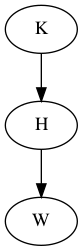
\includegraphics[height=0.5\textheight]{graphics/karma_chain}
\end{figure}

Then $P(K, H, W) = P(K) \, P(H | K) P(W | H) $.

\begin{definition}
A DAG of the form above is called a \emph{chain}.
\end{definition}
\end{frame}


\begin{frame}
  \frametitle{Decomposition example: Karma and weight-lifting} 
  Suppose $X = (K, H, W)$ admits the graph
  \begin{figure}[ht]
    \centering
    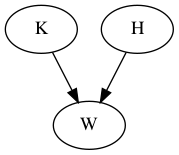
\includegraphics[height=0.5\textheight]{graphics/karma_collider}
  \end{figure}
  
  Then $P(K, H, W) = P(K) \, P(H) \, P(W | K, H)$.
  \begin{definition}
A DAG of the form above is called a \emph{collider} at $W$.
  \end{definition}
\end{frame}


\begin{frame}
\frametitle{Conditional independence}

Recall that two random variables $X, Y$ are \emph{independent} if $P(X=x, Y=y) = P(X=x) P(Y=y)$.

\begin{definition}
Let $X = (X_1, \ldots, X_m)$ be a probability distribution, and let $A, B, C$ be pair-wise disjoint subsets of ${1, \ldots, m}$, and define $X_A = (X_i)_{i \in A}$. Then $X_A, X_B$ are \emph{conditionally depenedent given $X_C$} if and only if 

\begin{align*}
P(&X_A = x_A,  \,X_B = x_B | X_C = x_c) \\
&= P(X_A = x_a | X_C = x_c) P(X_B = x_B | X_C = x_c)
\end{align*}

for all $x_A, x_B, x_C$.\newline
\end{definition}

For $X_A, X_B$ conditionally independent given $X_C$, we write $(X_A \ci X_B | X_C)$. See e.g. \cite{drton2008lectures} for a precise formulation.
\end{frame}

\begin{frame}
\frametitle{Conditional independence and d-separation teaser}
First example of discrete geometry helping statistics: conditional independence in a DAG model $(X, G)$ can be detected in properties of $G$\footnote{The required graph properties are combinatorial, but can also be understood geometrically, see e.g. \cite{drton2008lectures}.}. More precisely,


\begin{theorem}
If $(X, G)$ is a DAG model, then d-separation implies conditional independence.
\end{theorem}
See e.g. \cite{pearl2016causal}, chapter 2.
\end{frame}


\begin{frame}
\frametitle{More definitions before d-separation}

\begin{figure}[ht]
  \begin{tabular}{c}
    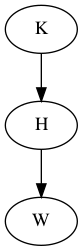
\includegraphics[height=0.35\textheight]{graphics/karma_chain}
  \end{tabular}
  \caption{Chain}
  \begin{tabular}{cc}
    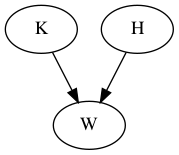
\includegraphics[height=0.35\textheight]{graphics/karma_collider}      
    &
    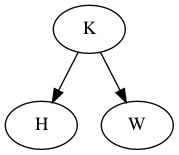
\includegraphics[height=0.35\textheight]{graphics/karma_fork}
  \end{tabular}
\caption{Collider at $W$, Fork at $K$}
\end{figure}

\end{frame}


\begin{frame}
\frametitle{d-separation in DAGs}
\begin{definition}
An undirected path $p$ in a DAG $G$ is \emph{blocked} by a set of nodes $C$ if and only if
\begin{enumerate}
\item $p$ contains a chain of nodes $X \to Y \to Z$, or a fork $X \rightarrow Y \leftarrow Z$ such that $Y \in C$, or
\item $p$ contains a collider $X \to Y \leftarrow Z$ such that $Y \notin C$ and descendant of $Y$ is in $C$.
\end{enumerate}
\end{definition}

\begin{definition}
If $C$ blocks every path between two nodes $X$ and $Y$, then $X$ and $Y$ are called \emph{d-separated conditional on $C$}, and we write 
$$(X \ci Y | C)_{G}$$.
\end{definition}

By the d-separation teaser theorem, $(X \ci Y | C)_{G}$ implies conditional independence.\newline
\end{frame}


\begin{frame}
\frametitle{d-separation example: hit rate for insurance}
\begin{figure}[ht]
  \centering
  \includegraphics[height=0.5\textheight]{graphics/hit}
\end{figure}

All paths from $\mathrm{product\_type}$ to $\mathrm{hit}$ are blocked by $\{\mathrm{days}, \mathrm{rating}\}$, hence $(\mathrm{product\_type} \ci \mathrm{hit} | \mathrm{days}, \mathrm{rating})_G$.
\end{frame}


\begin{frame}
\frametitle{Probability polytopes}

\emph{Goal}: Use geometric interpretation of multivariate discrete random variables to generate intersting fake data with few(er) parameters.\newline

Example: The family of all $X \sim Bernoulli$ can be represented as

\begin{equation*}
\Delta_1 = \{(p_0, p_1): p_i \geq 0, \sum p_i = 1\} \subseteq R^2\newline
\end{equation*}

Example: Consider the collider graph for Karma-influenced weight-lifting $(K, H, W)$. Then all possible conditional probability tables for $(W | K, H)$ can be parametrized as 

\begin{equation*}
  \{(p_{w | k, h}): p_{w | k, h} \geq 0, \sum_w p_{w  | k,h} = 1 \textrm{ for } (k, h) \in \{0, 1\}^2\} \subseteq R^8
\end{equation*}

In general, the space of multivariate discrete random variable distributions is a \emph{polytope}, see e.g. \cite{drton2008lectures}, Ch. 1.
\end{frame}


\begin{frame}
\frametitle{H- and V-representations of polytopes}

\begin{definition}
An \emph{H-polyhedron} is an intersection of closed halfspaces, i.e. a set $P \subseteq R^d$ presented in the form
\begin{equation*}
P = P(A,z)=\{ x \in R^d: Ax \leq z\} \textrm{ for some } A \in R^{m d}, z \in R^m.
\end{equation*}
\end{definition}

If $P$ is bounded (i.e. compact), then it is called a \emph{polytope}.

\begin{definition}
(Informal) A \emph{V-polytope} is the convex hull of a finite set of vertices $conv(V) \in R^d$. See \cite{ziegler2012lectures} for a precise definition.
\end{definition}

Example: The V-representation for all $Bernoulli$ distributions is
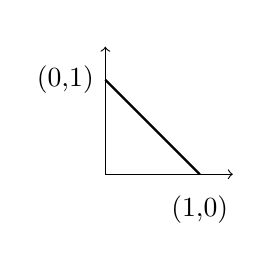
\begin{tikzpicture}[scale=1.2]
  % Draw axes
  \draw [<->] (0,1.35) node (yaxis) [above] {}
      |- (1.35,0) node (xaxis) [right] {};
  \draw [thick] (0,1.0) coordinate (b_1) node[anchor=west, xshift=-1.0cm] {(0,1)} -- (1.0,0) coordinate (b_2) node[anchor=south, yshift=-0.75cm] {(1,0)};
  
\end{tikzpicture}
\end{frame}


\begin{frame}
\frametitle{The main theorem of polytopes}

\begin{theorem}
  A subset $P \subset R^d$ is the convex hull of a finite point set (a \emph{V-polytope}) 
  \begin{equation*}
    P = conv(V) \textrm{ for some }V \in R^{dn}
  \end{equation*}
if and only if it is a bounded intersection of halfspaces (an \emph{H-polytope}) 
\begin{equation*}
  P = P(A,z) \textrm{ for some }A \in R^{md}, z \in R^m
\end{equation*}
\end{theorem}

See \cite{ziegler2012lectures} for a proof.\newline
\end{frame}


\begin{frame}
  \frametitle{Applying the main theorem to conditional probability tables}
For the Karma weight-lifting example, all conditional probability tables for $(W | K, H)$ that satisfy $E(W | K = 0) = 0$ (bad Karma, no weight) and $E(W | H = 0)=0.2$ can be written as an $H-polytope$ as above with additional constraints

\begin{align*}
\sum_{w, h} w \, p_{w | 0, h} &= 0\\
\sum_{w, k} w \, p_{w | k, 0} & = 0.2\newline
\end{align*}

By converting this H-representation to a V-representation, we can generate random conditional probability tables subject to expectation constrains.\newline

For an example, see the implementation of \href{https://munichpavel.github.io/fake-data-docs/html/\_modules/fake\_data\_for\_learning/utils.html\#ProbabilityPolytope}{ProbabilityPolytope} of \href{https://munichpavel.github.io/fake-data-for-learning/}{https://munichpavel.github.io/fake-data-for-learning/}.

\end{frame}


\begin{frame}[allowframebreaks]
    \frametitle{References}
    \setbeamertemplate{bibliography item}[text]
    \bibliographystyle{amsalpha}
    \bibliography{../references.bib}
\end{frame}

\end{document}